\section{Theory}
	Each atom in an equilibrium crystal lattice is precisely positioned at its lattice location. The morse potential, which has the lowest energy at the bond length internuclear distance when the lattice is in equilibrium, gives the potential energy for two particles. The lattice vibrations can be approximated to that of a harmonic oscillator in its most stable state, as seen in the image below. As a result, the lattice may be described as a spring and mass system, with atoms acting as the mass. As a result, when the atoms are pushed by a little amount from the equilibrium point, they tend to return to their original location. Due to interparticle interactions, these movements are subsequently imparted to all atoms, resulting in lattice vibrations.

	\begin{figure}[h]
		\centering
		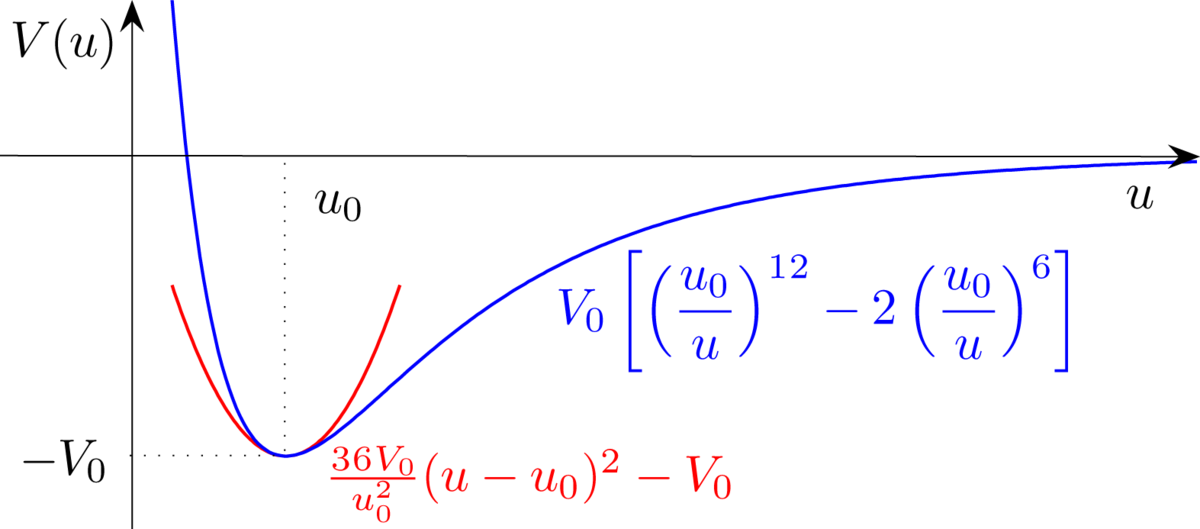
\includegraphics[width=0.9\columnwidth]{images/theory1.png}
		\caption{Harmonic Approximation for Lattice
		Dynamics}
		\label{fig:theory1}
	\end{figure}

	\begin{figure}[h]
		\centering
		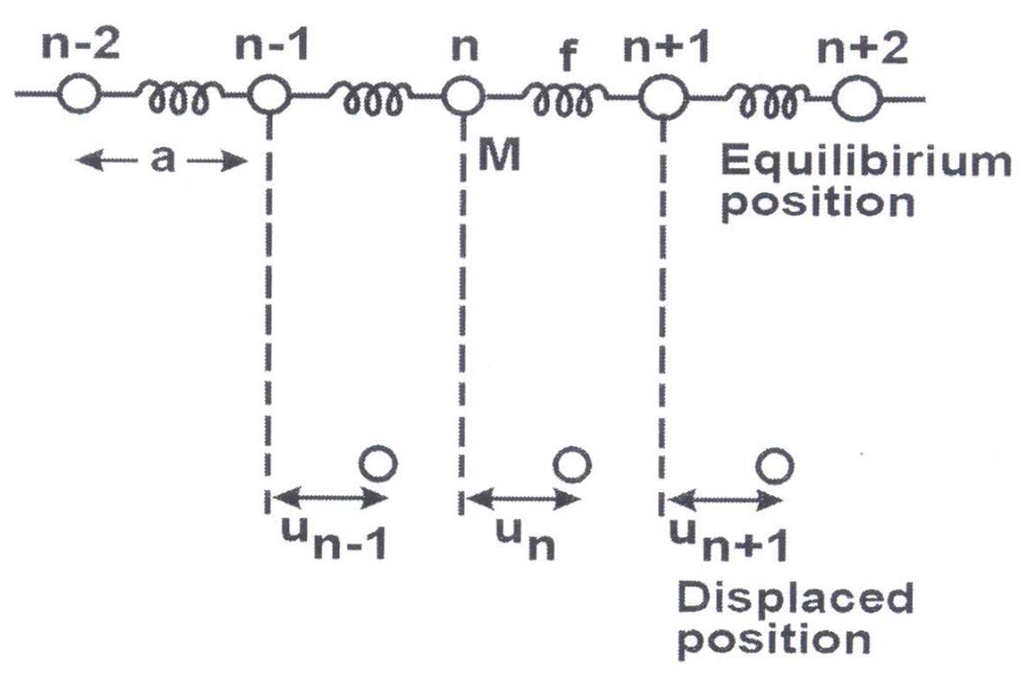
\includegraphics[width=0.9\columnwidth]{images/theory2.png}
		\caption{Spring Mass model of One Dimentional Linear Mono-atomic Lattice}
		\label{fig:theory2}
	\end{figure}

	\subsection{Monatomic Lattice Vibrrations}

		The harmonic approximation for a monoatomic crystal lattice is shown in \hyperref[fig:theory2]{Figure 2}. In \hyperref[fig:theory2]{Figure 2} these are the relevant constants:
		\begin{itemize}
			\item \textbf{a} $\rightarrow$ Lattice Constant
			\item \textbf{f} $\rightarrow$ Force constant
			\item \textbf{M} $\rightarrow$ Mass of the atom
		\end{itemize}

		On applying Newton's second law of motion and Hook's law for the sprin-mass system, we get the differential equation for the $n^{th}$ atom:

		\begin{equation}
			m \frac{d^2U_n}{dt^2} = f(U_{n+1} - 2U_n + U_{n-1})
			\label{eqn:1}
		\end{equation}

		where f corresponds to the force constant and $U_n$ is the displacement of the $n^{th}$ atom. Similarly, for $N$ number of particles at equilibrium particle distance $r$, there will $n$ coupled differential equations. Resonance would occur for the relation between length of the atomic chain in one dimension $(L = (N+1)r)$ and the wavelength of vibration, for an integer $m$ given as $2L = m\lambda$.
		
		Now, let us assume that the solution be of the form $U_n = A \exp(kx_n-\omega t)$. Substituting this in the differential equation with the boundary conditions of $x_N = x_0 = 0$, we get the following equation:

		$$\omega = \sqrt{\frac{4f}{m}}\abs{\;\sin\frac{ka}{2}}$$

		This is the dispersion relation, with $k$ denoting the $\sfrac{wavenumber}{wavevector}$. The Brilluoin zone for the newest (the independent values of $k$, values for which are indentical to other zones in the lattice) is supplied by the sin term as:

		$$\frac{-\pi}{a}\leq k \leq \frac{\pi}{a}$$
		$$\nu_{max} = \frac{1}{\pi}\sqrt{\frac{f}{m}}$$

	\subsection{Electrical Analogue of Monoatomic Lattice Vibrations}

		The electronic circuit that is an equivalent for these monoatomic vibration is that on an LC low pass filter as shown in figure, the output voltage of which is measured around the capacitor.

		On solving for the current arcoss the n-th capacitor, we find a differntial equation similar to that of \hyperref[eqn:1]{Equation 1} given as:

		$$C\frac{d^2V_n}{dt^2} = \frac{1}{L}(V_{n+1} - 2V_n + V_{n-1})$$

		where capacitance $C$ is equivalent to the mass, inductance $L$ to $\sfrac{1}{force constant}$, and $V_i$ is the voltage across the $i^{th}$ capacitor. Similar solution leads us to the equations of 		the dispersion equation and the cut off frequency which is equivalent to substituting the corresponding values of their electrical analogue.

		
		$$\omega = \sqrt{\frac{4}{LC}}\abs{\sin\theta}$$
		\begin{equation}
			v_{max} = \frac{1}{\pi\sqrt{LC}}
			\label{eqn:2}
		\end{equation}

		Where $\theta$ is the phase change introduced by the ach of the filter. By measuring the phase difference between the input and output voltages of the circuit as the function of frequency, the dispersion relation may be verified.

		\begin{figure}[h]
			\centering
			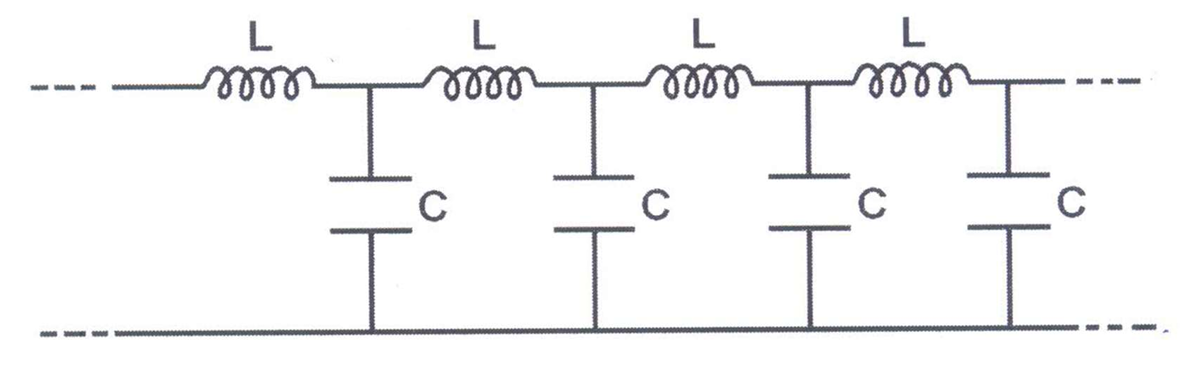
\includegraphics[width=0.9\columnwidth]{images/circ1.png}
			\caption{Monatomic lattice Analogous Circuit}
			\label{fig:circ1}
		\end{figure}

	\subsection{Diatomic Lattice Vibrations}
		For the diatomic case, the model (shown in \hyperref[fig:theory2]{Figure 2}) is changed ever so slightly. Here we have atoms of alternating masses $m$ and $M$ aligned in a row with lattice parameter $a$, and force constant $f$. The design is illustrated in \hyperref[fig:theory3]{Figure 3}.

		\begin{figure}[h]
			\centering
			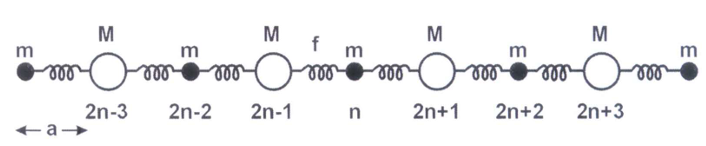
\includegraphics[width=0.9\columnwidth]{images/theory3.png}
			\caption{Diatomic lattice}
			\label{fig:theory3}
		\end{figure}

		Thus the coupled differential equations for the $n^{th}$ atom are given as:

		\begin{equation}
			m \frac{d^2U_n}{dt^2} = f(U_{n+1} - 2U_n + U_{n-1})
			\label{eqn:3}
		\end{equation}

		\begin{equation}
			M \frac{d^2U_{n+1}}{dt^2} = f(U_{n+2} - 2U_{n+1} + U_{n})
			\label{eqn:4}
		\end{equation}

		Solving the \hyperref[eqn:3]{Equation 3} and \hyperref[eqn:4]{Equation 4} we obtain:

		$$\omega = f\left(\frac{1}{m}+\frac{1}{M}\right)\pm f\sqrt{\left(\frac{1}{m}+\frac{1}{M}\right)^2 - 4 \frac{\sin^2ka}{mM}} $$

		As seen in the image above, the lower curve is known as the acoustic branch, while the top curve is known as the optical branch. The optical branch starts at $k = 0$ and ends at $\omega = 0$. The frequency then rises in a linear way as $k$ grows. This is why this branch is known as acoustic: it relates to elastic waves or sound at lower frequencies. Near the cut off frequency, this curve eventually saturates at the boundary of the Brillouin zone. At $k = 0$, the optical branch has a nonzero frequency. It has a higher frequency and is created as a result of vibrations caused by electromagnetic waves; the frequency is in the infrared region.

		For acoustic brach at $k = \omega = 0$, the relation between the amplitude of oscillation of the two particles is given as $A_1 = A_2 \cdot n$. Therefore the molecule oscillates as a rigid body for the acoustic mode. For the optical vibrations, it yeilds the relation $mA_1 + MA_2 = 0$. This implies that the optical oscillation takes place in such a way that the center of mass of a molecule remains fixed.

		\begin{figure}[h]
			\centering
			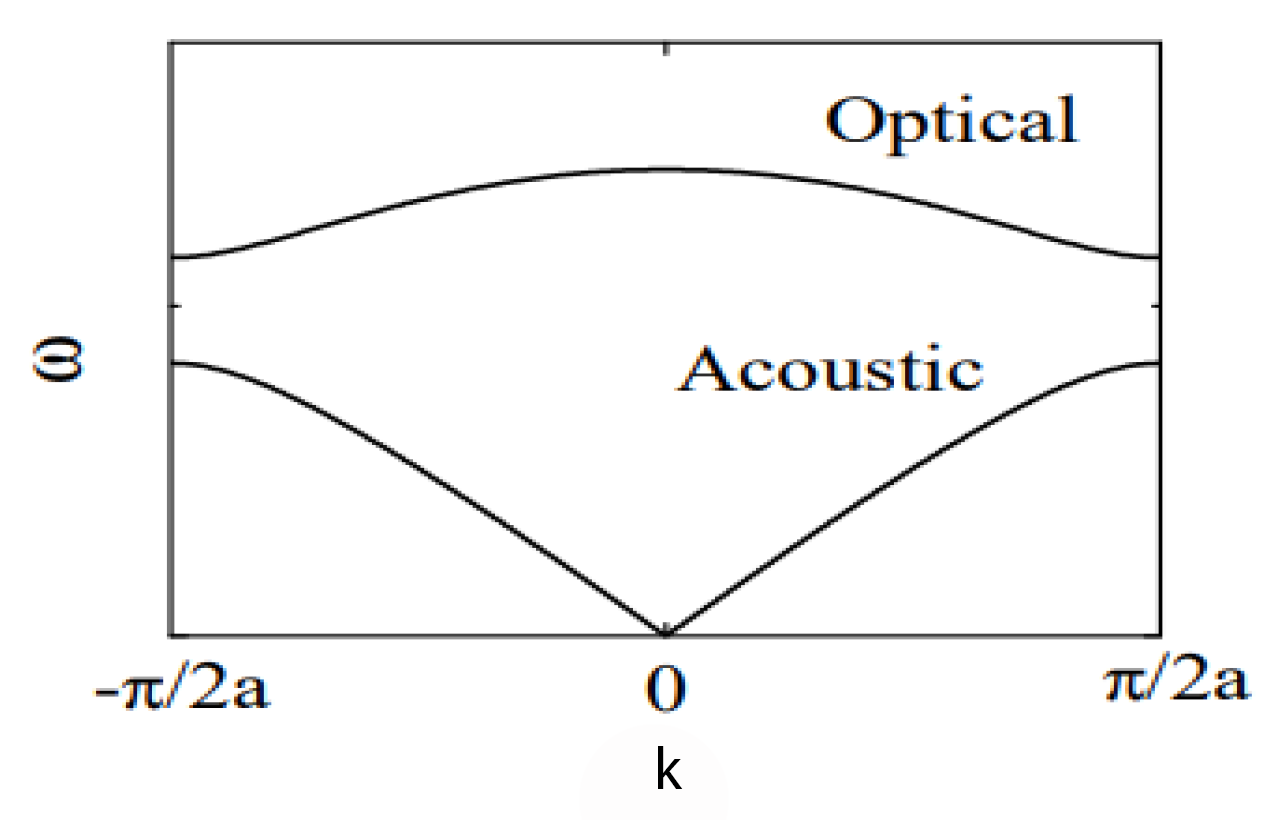
\includegraphics[width=0.9\columnwidth]{images/theory4.png}
		\end{figure}

		The electronic analogue for the circuit is given as shown with one unit cell comprising of two capacitors of capacitance $C$ and $C_1$ which acts as a band stop filter, where the gap is dependent on the $\frac{C}{C_1} \leftrightarrow \frac{m}{M}$. The analogous dispersion relation is given as:

		$$\omega = \frac{1}{L}\left(\frac{1}{C}+\frac{1}{C_1}\right)\pm \frac{1}{L}\sqrt{\left(\frac{1}{C}+\frac{1}{C_1}\right)^2 - 4 \frac{\sin^2\theta}{CC_1}}$$

		On putting $k = \pm\pi$, we can obtain the range of the band gap, which lies between:

		\begin{equation}
			\nu_{upperbound} = \frac{1}{2\pi\sqrt{LC}}
			\label{eqn:5}
		\end{equation}

		\begin{equation}
			\nu_{lowerbound} = \frac{1}{2\pi\sqrt{LC_1}}
			\label{eqn:6}
		\end{equation}

		\begin{figure}[h]
			\centering
			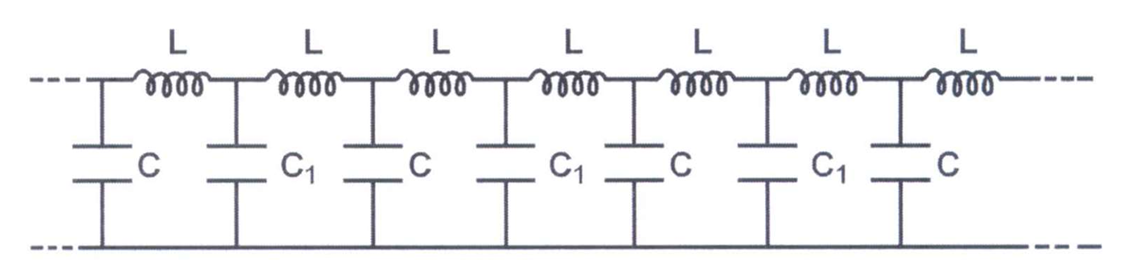
\includegraphics[width=0.9\columnwidth]{images/circ2.png}
			\caption{Diatomic lattice Analogous Circuit}
			\label{fig:circ2}
		\end{figure}